\documentclass[11pt,a4paper]{article}
\usepackage[utf8]{inputenc}
\usepackage{amsmath}
\usepackage{graphicx}
\usepackage{float}
\usepackage{physics}
\usepackage{listings} 
\usepackage{xcolor}
\usepackage{tikz}
\usepackage{geometry}
\usepackage{hyperref}
\hypersetup{
    colorlinks=true,
    linkcolor=blue,
    filecolor=magenta,      
    urlcolor=cryan,
}
\urlstyle{same}
\geometry{
    a4paper,
    total={180mm, 260mm},
    left=20mm,
    top=10mm,
}
\usepackage[T1]{fontenc}

\definecolor{codegreen}{rgb}{0,0.6,0}
\definecolor{codegray}{rgb}{0.5,0.5,0.5}
\definecolor{codepurple}{rgb}{0.58,0,0.82}
\definecolor{backcolour}{rgb}{0.95,0.95,0.92}

\lstdefinestyle{mystyle}{
    backgroundcolor=\color{backcolour},
    commentstyle=\color{codegreen},
    keywordstyle=\color{magenta},
    numberstyle=\tiny\color{codegray},
    stringstyle=\color{codepurple},
    basicstyle=\ttfamily\footnotesize,
    breakatwhitespace=false,
    breaklines=true,
    captionpos=b,
    keepspaces=true,
    numbers=left,
    numbersep=5pt,
    showspaces=false,
    showstringspaces=false,
    showtabs=false,
    tabsize=2
}
\lstset{style = mystyle}

\title{Computer Architecture HW3}
\author{Tony G. Liu B05202068}

\begin{document}
    \maketitle
    
\section{ALU}%
\label{sec:ALU}

\begin{itemize}
    \item Signed Add: Overflow condition- \texttt{\{a[MSB]+b[MSB], (a+b)[MSB]\}==  2'b10, 2'b01 }\n
        
    \item Signed Sub: Overflow condition- \texttt{\{a[MSB]-b[MSB], (a-b)[MSB]\}==  2'b01, 2'b10 }\n

    \item Signed Mul: Overflow condition- \texttt{\{a[MSB] \string^ b[MSB], (a*b)[MSB]\}==  2'b00, 2'b11}\n

    \item Signed Max/Min: Take the \texttt{\$signed(..)} before comparing two numbers.\n 

    \item Unsigned Add: Overflow condition- \texttt{\{a[MSB]+b[MSB], (a+b)[MSB]\}==  2'b00(a[MSB],b[MSB] == 1), 2'b10 }\n


    \item Unsigned Sub:   Overflow condition- \texttt{a < b}
    \item Unsigned Mul: Overflow condition- the sum of the leftmost set bit position of \texttt{a} and \texttt{b} is over $31$

    \item Unsigned Max/Min: Simpley do the comparison\n

    \item And:  \texttt{a \& b}

    \item Or:   \texttt{a | b}

    \item Xor:  \texttt{a \string^ b}

    \item BitFlip: \texttt{\string~a }

    \item BitReverse: Keep putting the set bits of \texttt{a} in the output until \texttt{a} becomes zero. After \texttt{a} becomes zero, shift the remaining bits of the output by the number of count. It takes $O(\log n)$ time complexity.  
\end{itemize}


\section{FPU}%
\label{sec:FPU}

\subsection{Add}%
\label{sub:Add}

\hspace{0.6cm}1. Sort the two numbers \texttt{i\_data\_a} and \texttt{i\_data\_b} so that the first operand  \texttt{a} is no less than the second operand \texttt{b}.  \n

2. Do the number alignment: \n
    \begin{itemize}
        \item Get the exponent difference \texttt{exp\_diff}
        \item Right shift the significand of \texttt{b} by the exponent difference and increment the exponent of \texttt{b} by the difference 
    \end{itemize}\n

3. \texttt{OR} the last \texttt{exp\_diff} $- 1 $ bits of significand  \texttt{b} and let it be \texttt{S}\n

4. Add significand \texttt{a} and the shifted significand \texttt{b} if their sign are the same, subtract if otherwise.\n

5. Check the carry bit of the significand \texttt{sig\_add} after adding.\n

6. \texttt{R} would be the bit right after the LSB of \texttt{sig\_add}, and \texttt{S} will be the \texttt{OR} of rest of the remaining bits.\n

7. Increment or decrement the amswer by $1$(depending on the sign bits) if the bits \texttt{ \{R, S\} == 2'b11, 2b'10}\n

\subsection{Multiplication}%
\label{sub:Multiplication}

\hspace{0.6cm}1. Take the product of two significands of \texttt{i\_data\_a} and \texttt{i\_data\_b}.\n

2. \texttt{OR} the last $32$ bits of the product and let it be \texttt{S}(= \texttt{sig\_product[31:0]} )\n

3. Do the normalization($i.e.$, check the MSB of the product)\n

4. Take the first $32$ bits of the product and plus  \texttt{sig\_product[32]\&S}\n

5. Add the two exponent and minus $127$. Increment by  $1$ if the normalization bit is set.\n 

6. Putting the sign bit, \texttt{sig\_product} and the exponent result together.
\section{CPU}%
\label{sec:CPU}
    
    The block diagram is mostly the same as the one in textbook, except that we have to wait for several cycles for the data in instruction memory and data memory to be ready. 
    \begin{figure}[htpb]
        \centering
        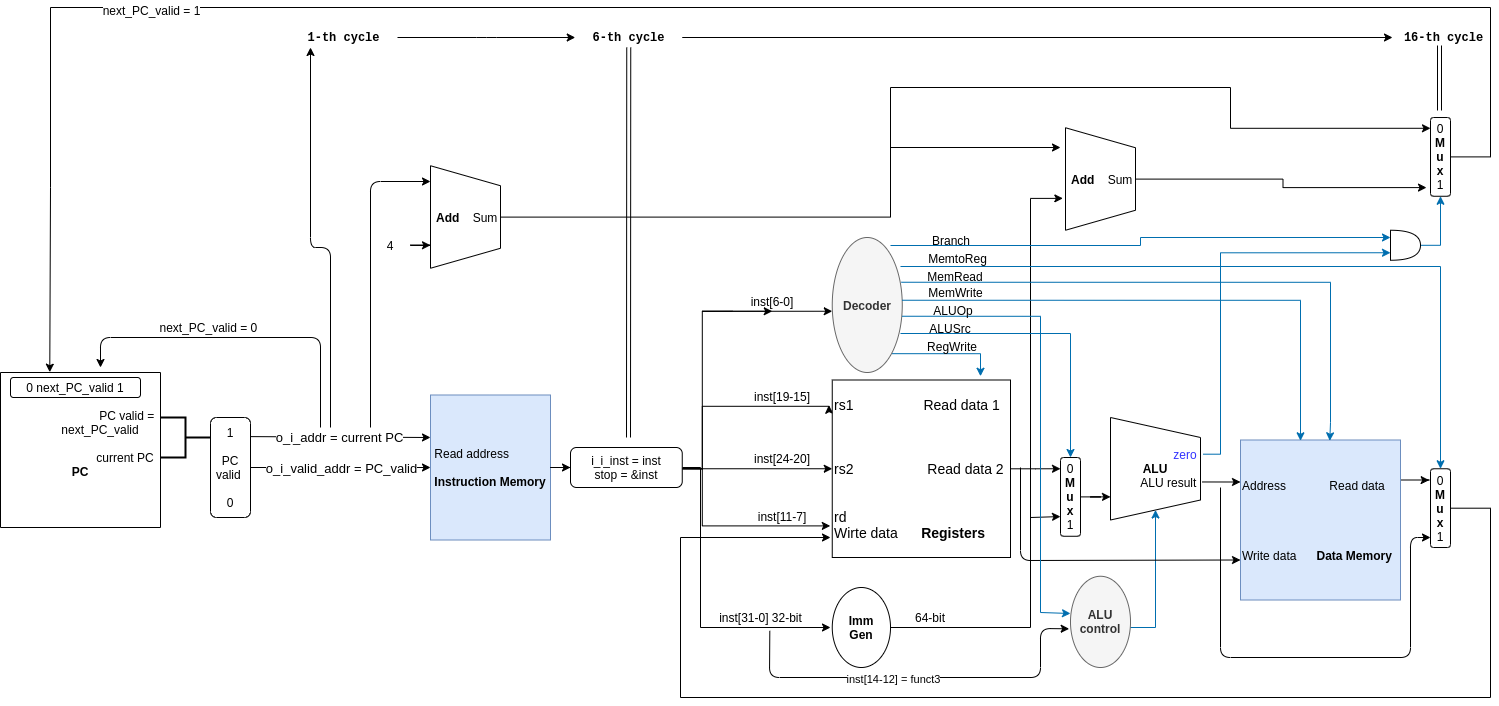
\includegraphics[width=1.0\textwidth]{../CPU_block_diagram.png}
    \end{figure}

\end{document}
